% Options for packages loaded elsewhere
\PassOptionsToPackage{unicode}{hyperref}
\PassOptionsToPackage{hyphens}{url}
%
\documentclass[
  12pt,
]{article}
\usepackage{lmodern}
\usepackage{setspace}
\usepackage{amssymb,amsmath}
\usepackage{ifxetex,ifluatex}
\ifnum 0\ifxetex 1\fi\ifluatex 1\fi=0 % if pdftex
  \usepackage[T1]{fontenc}
  \usepackage[utf8]{inputenc}
  \usepackage{textcomp} % provide euro and other symbols
\else % if luatex or xetex
  \usepackage{unicode-math}
  \defaultfontfeatures{Scale=MatchLowercase}
  \defaultfontfeatures[\rmfamily]{Ligatures=TeX,Scale=1}
\fi
% Use upquote if available, for straight quotes in verbatim environments
\IfFileExists{upquote.sty}{\usepackage{upquote}}{}
\IfFileExists{microtype.sty}{% use microtype if available
  \usepackage[]{microtype}
  \UseMicrotypeSet[protrusion]{basicmath} % disable protrusion for tt fonts
}{}
\makeatletter
\@ifundefined{KOMAClassName}{% if non-KOMA class
  \IfFileExists{parskip.sty}{%
    \usepackage{parskip}
  }{% else
    \setlength{\parindent}{0pt}
    \setlength{\parskip}{6pt plus 2pt minus 1pt}}
}{% if KOMA class
  \KOMAoptions{parskip=half}}
\makeatother
\usepackage{xcolor}
\IfFileExists{xurl.sty}{\usepackage{xurl}}{} % add URL line breaks if available
\IfFileExists{bookmark.sty}{\usepackage{bookmark}}{\usepackage{hyperref}}
\hypersetup{
  pdftitle={sampbias, a method for quantifying geographic sampling biases in species distribution data},
  hidelinks,
  pdfcreator={LaTeX via pandoc}}
\urlstyle{same} % disable monospaced font for URLs
\usepackage[margin=1in]{geometry}
\usepackage{color}
\usepackage{fancyvrb}
\newcommand{\VerbBar}{|}
\newcommand{\VERB}{\Verb[commandchars=\\\{\}]}
\DefineVerbatimEnvironment{Highlighting}{Verbatim}{commandchars=\\\{\}}
% Add ',fontsize=\small' for more characters per line
\usepackage{framed}
\definecolor{shadecolor}{RGB}{248,248,248}
\newenvironment{Shaded}{\begin{snugshade}}{\end{snugshade}}
\newcommand{\AlertTok}[1]{\textcolor[rgb]{0.94,0.16,0.16}{#1}}
\newcommand{\AnnotationTok}[1]{\textcolor[rgb]{0.56,0.35,0.01}{\textbf{\textit{#1}}}}
\newcommand{\AttributeTok}[1]{\textcolor[rgb]{0.77,0.63,0.00}{#1}}
\newcommand{\BaseNTok}[1]{\textcolor[rgb]{0.00,0.00,0.81}{#1}}
\newcommand{\BuiltInTok}[1]{#1}
\newcommand{\CharTok}[1]{\textcolor[rgb]{0.31,0.60,0.02}{#1}}
\newcommand{\CommentTok}[1]{\textcolor[rgb]{0.56,0.35,0.01}{\textit{#1}}}
\newcommand{\CommentVarTok}[1]{\textcolor[rgb]{0.56,0.35,0.01}{\textbf{\textit{#1}}}}
\newcommand{\ConstantTok}[1]{\textcolor[rgb]{0.00,0.00,0.00}{#1}}
\newcommand{\ControlFlowTok}[1]{\textcolor[rgb]{0.13,0.29,0.53}{\textbf{#1}}}
\newcommand{\DataTypeTok}[1]{\textcolor[rgb]{0.13,0.29,0.53}{#1}}
\newcommand{\DecValTok}[1]{\textcolor[rgb]{0.00,0.00,0.81}{#1}}
\newcommand{\DocumentationTok}[1]{\textcolor[rgb]{0.56,0.35,0.01}{\textbf{\textit{#1}}}}
\newcommand{\ErrorTok}[1]{\textcolor[rgb]{0.64,0.00,0.00}{\textbf{#1}}}
\newcommand{\ExtensionTok}[1]{#1}
\newcommand{\FloatTok}[1]{\textcolor[rgb]{0.00,0.00,0.81}{#1}}
\newcommand{\FunctionTok}[1]{\textcolor[rgb]{0.00,0.00,0.00}{#1}}
\newcommand{\ImportTok}[1]{#1}
\newcommand{\InformationTok}[1]{\textcolor[rgb]{0.56,0.35,0.01}{\textbf{\textit{#1}}}}
\newcommand{\KeywordTok}[1]{\textcolor[rgb]{0.13,0.29,0.53}{\textbf{#1}}}
\newcommand{\NormalTok}[1]{#1}
\newcommand{\OperatorTok}[1]{\textcolor[rgb]{0.81,0.36,0.00}{\textbf{#1}}}
\newcommand{\OtherTok}[1]{\textcolor[rgb]{0.56,0.35,0.01}{#1}}
\newcommand{\PreprocessorTok}[1]{\textcolor[rgb]{0.56,0.35,0.01}{\textit{#1}}}
\newcommand{\RegionMarkerTok}[1]{#1}
\newcommand{\SpecialCharTok}[1]{\textcolor[rgb]{0.00,0.00,0.00}{#1}}
\newcommand{\SpecialStringTok}[1]{\textcolor[rgb]{0.31,0.60,0.02}{#1}}
\newcommand{\StringTok}[1]{\textcolor[rgb]{0.31,0.60,0.02}{#1}}
\newcommand{\VariableTok}[1]{\textcolor[rgb]{0.00,0.00,0.00}{#1}}
\newcommand{\VerbatimStringTok}[1]{\textcolor[rgb]{0.31,0.60,0.02}{#1}}
\newcommand{\WarningTok}[1]{\textcolor[rgb]{0.56,0.35,0.01}{\textbf{\textit{#1}}}}
\usepackage{longtable,booktabs}
% Correct order of tables after \paragraph or \subparagraph
\usepackage{etoolbox}
\makeatletter
\patchcmd\longtable{\par}{\if@noskipsec\mbox{}\fi\par}{}{}
\makeatother
% Allow footnotes in longtable head/foot
\IfFileExists{footnotehyper.sty}{\usepackage{footnotehyper}}{\usepackage{footnote}}
\makesavenoteenv{longtable}
\usepackage{graphicx,grffile}
\makeatletter
\def\maxwidth{\ifdim\Gin@nat@width>\linewidth\linewidth\else\Gin@nat@width\fi}
\def\maxheight{\ifdim\Gin@nat@height>\textheight\textheight\else\Gin@nat@height\fi}
\makeatother
% Scale images if necessary, so that they will not overflow the page
% margins by default, and it is still possible to overwrite the defaults
% using explicit options in \includegraphics[width, height, ...]{}
\setkeys{Gin}{width=\maxwidth,height=\maxheight,keepaspectratio}
% Set default figure placement to htbp
\makeatletter
\def\fps@figure{htbp}
\makeatother
\setlength{\emergencystretch}{3em} % prevent overfull lines
\providecommand{\tightlist}{%
  \setlength{\itemsep}{0pt}\setlength{\parskip}{0pt}}
\setcounter{secnumdepth}{-\maxdimen} % remove section numbering
\usepackage{caption}
\usepackage{fancyhdr}
\pagestyle{fancy}
\fancyhead[L]{Quantifying sampling biases}
\fancyhead[R]{\thepage}
\fancyfoot{}
\usepackage{float}
\floatplacement{figure}{H}
\usepackage{lineno}
\linenumbers
\usepackage[url=false]{biblatex}
\usepackage{setspace}

\title{sampbias, a method for quantifying geographic sampling biases in species distribution data}
\author{}
\date{\vspace{-2.5em}}

\begin{document}
\maketitle

\setstretch{2}
\newpage{}

\hypertarget{abstract}{%
\section{Abstract}\label{abstract}}

Geo-referenced species occurrences from public databases have become essential to biodiversity research and conservation. However, geographical biases are widely recognized as a factor limiting the usefulness of such data for understanding species diversity and distribution. In particular, differences in sampling intensity across a landscape due to differences in human accessibility are ubiquitous but may differ in strength among taxonomic groups and data sets. Although several factors have been described to influence human access (such as presence of roads, rivers, airports and cities), quantifying their specific and combined effects on recorded occurrence data remains challenging. Here we present \emph{sampbias}, an algorithm and software for quantifying the effect of accessibility biases in species occurrence data sets. \emph{sampbias} uses a Bayesian approach to estimate how sampling rates vary as a function of proximity to one or multiple bias factors. The results are comparable among bias factors and data sets. We demonstrate the use of \emph{sampbias} on a data set of mammal occurrences from the island of Borneo, showing a high biasing effect of cities and a moderate effect of roads and airports. \emph{sampbias} is implemented as a well-documented, open-access and user-friendly R package that we hope will become a standard tool for anyone working with species occurrences in ecology, evolution, conservation and related fields.

\hypertarget{keywords}{%
\section{Keywords}\label{keywords}}

Collection effort, Global Biodiversity Information Facility (GBIF), Presence only data, Roadside bias, Sampling intensity

\newpage{}

\hypertarget{background}{%
\section{Background}\label{background}}

Publicly available data sets of geo-referenced species occurrences, such as provided by the Global Biodiversity Information Facility (www.gbif.org) have become a fundamental resource in biological sciences, especially in biogeography, conservation, and macroecology. However, these data sets are typically not collected systematically and rarely include information on collection effort. Instead, they are often compiled from a variety of sources (e.g., scientific expeditions, census counts, genetic barcoding studies and citizen-science observations). Species occurrences are therefore often subject to multiple sampling biases (Meyer et al. 2016).

Sampling biases that may affect the recording of species occurrences (presence, absence and abundance, Isaac and Pocock 2015, Boakes et al. 2010) include the under-sampling of specific taxa (``taxonomic bias'', e.g., birds \emph{vs.} nematodes), specific geographic regions (``geographic bias'', e.g., easily accessible \emph{vs.} remote areas), and specific temporal periods (``temporal bias'', e.g., wet \emph{vs.} dry season). In particular geographic sampling bias---the fact that sampling effort is spatially biased, rather than equally distributed over the study area---is likely to be widespread in all non-systematically collected data sets of species distributions.

Many aspects can lead to sampling biases, including socio-economic factors (e.g., national research spending, history of scientific research; Zizka et al. 2020, Meyer et al. 2015, Daru et al. 2018), political factors (e.g., armed conflict, democratic rights; Rydén et al. 2020), and physical accessibility (e.g., distance to a road or river, terrain conditions, slope; Yang et al. 2014, Botts et al. 2011). Especially physical accessibility by people is omnipresent as a bias factor (e.g., Lin et al. 2015, Kadmon et al. 2004, Engemann et al. 2015), across spatial scales, as the commonly used term ``roadside bias'' testifies. In practice, this means that most species observations are made in or near cities, along roads, paths, rivers and near human settlements. Relatively fewer observations are expected to be available from inaccessible areas in e.g., a tropical rainforest or a mountain top. Since the recording of different taxonomic groups poses different challenges, geographic sampling bias and the effect of accessibility may differ among taxonomic groups (Vale and Jenkins 2012).

The implications of not considering geographic sampling biases in biodiversity research are likely substantial (Barbosa et al. 2013, Meyer et al. 2016, Yang et al. 2013). The presence of geographic sampling biases is broadly recognized (e.g., Kadmon et al. 2004), and approaches exist to account for it in some analyses---such as species-richness estimates (Engemann et al. 2015), occupancy models (Kery and Royle 2016), and abundance estimates (Shimadzu and Darnell 2015). In the case of species distribution modelling---the statistical estimation of species geographic distributions based on known occurrences and environmental conditions---geographically biased sampling is problematic because it often causes environmentally biased sampling which decreases model performance (Kadmon et al. 2004, Bystriakova et al. 2012, Lobo and Tognelli 2011, Kramer-Schadt et al. 2013, Varela et al. 2014). Many approaches exist to remedy the effect of biased sampling on species distribution models (Fourcade et al. 2014), including rarefaction to reduce clumped sampling in geographic (Beck et al. 2014, Aiello-Lammens et al. 2015, Boria et al. 2014) or environmental space (Varela et al. 2014), collecting background points for presence-only models to reflect the same sampling bias as the presence records (Phillips et al. 2009), and explicitly modelling sampling bias (Fithian et al. 2015, Stolar and Nielsen 2015, Komori et al. 2020). In contrast, few attempts have been made to compare the geographic sampling bias among data sets (Fernández and Nakamura 2015, Ruete 2015, Monsarrat et al. 2019) and to our knowledge, no tools exist to quantify the effect size of specific bias factors and compare it among them. We define as \textit{bias factors} any anthropogenic or natural features that facilitate human access and sampling, such as roads, rivers, airports, and cities.

It is unrealistic to expect that accessibility bias in biodiversity data will disappear even after more automated observation technologies are developed. It is therefore crucial that researchers realise the intrinsic biases associated with the data they deal with, especially in cross-taxonomic studies, since occurrence data sets from different taxa are likely differently affected by sampling biases due to differences in specimen collection and transportation. This is the first step towards estimating to which extent these biases may affect their analyses, results and conclusions. Any study dealing with species occurrence data should arguably assess the strength of accessibility biases in the underlying data. Such a quantification can also help researchers to target further sampling efforts.

Here, we present \emph{sampbias} v1.0.4, a probabilistic method to quantify accessibility bias in data sets of species occurrences. \emph{sampbias} is implemented as a user-friendly R-package and uses a Bayesian approach to address three questions:

\begin{enumerate}
\def\labelenumi{\arabic{enumi})}
\item
  How strong is the accessibility bias in a given data set?
\item
  How strong is the effect of different bias factors in causing the overall accessibility bias?
\item
  How is accessibility bias distributed in space?
\end{enumerate}

\emph{sampbias} is implemented in R (R Core Team 2019), based on commonly used packages for data handling (\texttt{ggplot}, Wickham 2009, \texttt{forcats}, 2019, \texttt{tidyr}, Wickham and Henry 2019, \texttt{dplyr}, Wickham et al. 2019, \texttt{magrittr}, Bache and Wickham 2014, \texttt{viridis}, Garnier 2018), handling geographic information and geo-computation (\texttt{raster}, Hijmans 2019, \texttt{sp}, Pebesma and Bivand 2005, Bivand et al. 2013) and statistical modelling (\texttt{stats}, R Core Team 2019). \emph{sampbias} offers an easy and largely automated means for biodiversity scientists and non-specialists alike to explore bias in species occurrence data, in a way that is comparable across data sets. The results may be used to identify priorities for further collection or digitalization efforts and to assess the reliability of scientific results based on publicly available species distribution data.

\hypertarget{methods-and-features}{%
\section{Methods and Features}\label{methods-and-features}}

\hypertarget{general-concept}{%
\subsection{General concept}\label{general-concept}}

Under the assumption that organisms occur across the entire area of interest, we can expect the number of sampled occurrences in a restricted area, such as a single biome, to be distributed uniformly in space (even though, of course, the density of individuals and the species diversity may be heterogeneous). With \emph{sampbias} we assess to which extent variation in sampling rates can be explained by distance from bias factors.

\emph{sampbias} works at a user-defined spatial scale, and any data set of multi-species occurrence records can be tested against any geographic gazetteer. Reliability increases with increasing data set size. Default global gazetteers for airports, cities, rivers and roads are provided with \emph{sampbias}, and user-defined gazetteers can be added easily. Species occurrence data as downloaded from the data portal of GBIF can be directly used as input data for \emph{sampbias}. The output of the package includes measures of the sampling rates across space, which are comparable between different gazetteers (e.g., comparing the biasing effect of roads and rivers), different taxa (e.g., birds \emph{vs.} flowering plants) and different data sets (e.g., specimens \emph{vs.} human observations).

\hypertarget{distance-calculation}{%
\subsection{Distance calculation}\label{distance-calculation}}

\emph{sampbias} uses gazetteers of the geographic location of bias factors (hereafter indicated with B) to generate a regular grid across the study area. By default the study area is defined by the geographic extent of the study data set, but it can also be customized via user-defined polygons, for instance to limit the analyses to an environmentally homogeneous region (e.g., a rainforest) or an area of special interest (e.g., a national park). In this case all occurrence records outside the user-defined area will be disregarded for the analysis.. For each grid cell \(i\), we then compute a vector \(X_i(j)\) of minimum distances (straight aerial distance, ``as the crow flies'') to each bias factor \(j \in B\). The resolution of the grid defines the precision of the distance estimates, for instance a \(1 \times 1\) degree raster will yield approximately a 110 km precision at the equator. Due to the assumption of homogeneous sampling and a computational trade-off between the resolution of the regular grid and the extent of the study area (for instance, a 1 second resolution for a global data set would become computationally prohibitive in most practical cases), \emph{sampbias} is best suited for local or regional data sets at high resolution (c.~100 -- 10,000 m). Since the differences in grid cell size are negligible on the local and regional scale, sampbias uses a latitude/longitude grid by default, but a custom grid in any projection and coordinate reference system---for instance an equal area grid, which is often more suitable for large spatial analyses---may be provided by the user.

\hypertarget{quantifying-accessibility-bias-using-a-bayesian-framework}{%
\subsection{Quantifying accessibility bias using a Bayesian framework}\label{quantifying-accessibility-bias-using-a-bayesian-framework}}

We describe the observed number of sampled occurrences \(S_i\) within each cell \(i\) as the result of a Poisson sampling process with rate \(\lambda_i\). We model the rate \(\lambda_i\) as a function of a parameter \(q\), which represents the expected number of occurrences per cell in the absence of biases, i.e.~when \(\sum_{j=1}^{B}{ X_i(j)} = 0\). Additionally, we model \(\lambda_i\) to decrease exponentially as a function of distance from bias factors, such that increasing distances will result in a lower sampling rate. For a single bias factor the rate of cell \(i\) with distance \(X_i\) from a bias is:
\[
\lambda_i = q \times \exp \left(- w X_i \right)
\]
where \(w \in \mathbb{R^+}\) defines the steepness of the Poisson rate decline, such that \(w \approx 0\) results in a null model of uniform sampling rate \(q\) across cells. In the presence of multiple bias factors (e.g., roads and rivers), the sampling rate decrease is a function of the cumulative effects of each bias and its distance from the cell:
\[
\lambda_i = q \times \exp \left(-\sum_{j=1}^{B}{w_j X_i(j)} \right) \ \ \ \ (1)
\]
where a vector \(\mathbf{w} = [w_1, ..., w_B]\) describes the amount of bias attributed to each specific factor.

To quantify the amount of bias associated with each factor, we jointly estimate the parameters \(q\) and \(\mathbf{w}\) in a Bayesian framework. We use Markov Chain Monte Carlo (MCMC) to sample these parameters from their posterior distribution:
\[
P(q, \mathbf{w} | \mathbf{S}) \propto \prod_{i=1}^{N}{ Poi(S_i | \lambda_i) } \times P(q) P(\mathbf{w}) \ \ \ \ (2)
\]
where the likelihood of sampled occurrences \(S_i\) within each cell \(Poi(S_i | \lambda_i)\) is the probability mass function of a Poisson distribution with rate per cell defined as in Eqn. (1). The likelihood is then multiplied across the \(N\) cells considered. We use exponential priors on the parameters \(q\) and \(\mathbf{w}\), \(P(q) \sim \Gamma(1, 0.01)\) and \(P(\mathbf{w}) \sim \Gamma(1, 1)\), respectively. We chose exponential priors because they represent the standard choice for rate parameters such as \(q\) and the weights \(\mathbf{w}\), all of which must be positive and have support {[}0, +inf{]}. We designed the priors to be informative (i.e.~not allowing negative values) and yet vague enough to encompass a much wider range of parameter space than the range of values observed in empirical tests. Custom priors, within the flexible family of gamma distributions, which include the exponential priors used here, are possible via the \texttt{prior\_q} and \texttt{prior\_w} arguments of the \texttt{calculate\_bias} function. Additionally, since the null expectation in the absence of biases is that the weights are close to 0, we implement a hierarchical model, in which the rate parameter of the gamma prior can be itself estimated from the data. Thus, we set \(P(\mathbf{w}) \sim \Gamma(a=1, b)\) and assign a vague hyper-prior on the rate \(P(b) \sim \Gamma(\alpha_0=1, \beta_0=0.001)\). The choice of a conjugate gamma hyper-prior allows us to sample the rate directly from its posterior distribution:
\[
b \sim \Gamma \left(\alpha_0 + a B,\ \beta_0  \sum_{j=1}^{B}{w_j} \right) \ \ \ \ (3)
\]
The use of a hyper-prior has the advantage of making the prior on the weights more flexible and able to adapt to different data sets reducing the need for user-defined arbitrary choices. Additionally, it works as a regularization technique reducing the risks of over-parametrization, by shrinking the weights around small values when there is no evidence in the data indicating a bias.

We summarize the parameters by computing the mean of the posterior samples and their standard deviation. We interpret the magnitude of the elements in \(\mathbf{w}\) as a function of the importance of the individual biases. We note, however, that this test is not explicitly intended to assess the significance of each bias factor. Because several bias factors might be correlated (e.g.~cities and airports), simply summing their effect from independent analyses would result in an overestimation of the total bias. It is therefore important to jointly estimate the effects of correlated factors, as this is based on the likelihood of the data given the combined effects of all biasing factors. A Bayesian variable selection method could be used to quantify the expected amount of bias in the data predicted by single or a particular combination of predictors, but falls beyond the scope of the current study. In the empirical example below we show, however, how a simple simulation can be used to asses whether the estimated bias factors significantly differ from a null expectation.

We summarize the results by mapping the estimated (the relative deviation of sampling rate from the maximum
sampling rate (or on user choice the estimated sampling rates, \(\lambda_i\)) across space. These rates represent the expected number of sampled occurrences for each grid cell and provide a graphical representation of the spatial variation of sampling rates. Provided that the cells are of equal size, the estimated rates will be comparable across data sets, regions, and taxonomic groups. Analysing different regions, biomes, or taxa in separate analyses allows to account for differences in sampling rates, which are not linked with bias factors. For instance, the unbiased sampling rate \(q\) is expected to differ between a highly sampled clade like birds and under-sampled groups of invertebrates, but their sampling biases (\(\mathbf{w}\)) might be similar across the two groups.

\hypertarget{example-and-empirical-validation}{%
\subsection{Example and empirical validation}\label{example-and-empirical-validation}}

A default \emph{sampbias} analysis can be run with few lines of code in R, based on a \texttt{data.frame} including species identity and geographic coordinates. The main function \texttt{calculate\_bias} creates an object of the class \texttt{"sampbias"}, for which the package provides a plotting and summary method. Additional options exist to provide custom gazetteers, study area, spatial grid and grain size of the analysis, as well as operators for the calculation of the bias distances, including priors for \(q\) and \(\mathbf{w}\). A tutorial on how to use \emph{sampbias} is available with the package and in the electronic supplement of this publication (Appendix S1).

To exemplify the use of \emph{sampbias}, we downloaded the occurrence records of all mammals available from the island of Borneo (n = 6,262, GBIF.org 2016) and ran \emph{sampbias} using the default gazetteers as shown in the example code below, to test the biasing effect of the main airports, cities and roads in the data set. The example data set is provided with \emph{sampbias}.

We found a strong effect of cities on sampling intensity, a moderate effect of roads and airports and a negligible effect of rivers (Fig. \ref{fig:empirical}). All models predict a low number of collection records in the centre of Borneo (Fig. \ref{fig:spatial}), which reflects the original data, and where accessibility means are low (Figure S1 in Appendix S2). The empirical example illustrates the use of \emph{sampbias}, for detailed analyses or a smaller geographic scale, higher resolution gazetteers, including smaller roads and rivers and a higher spatial resolution would be desirable. Results might change with increasing resolution, since roads and rivers might have a stronger effect on higher resolutions (facilitating most the access to their immediate vicinity), whereas cities and airports might have a stronger effect on the larger scale (facilitating access to a larger area).

\begin{Shaded}
\begin{Highlighting}[]
\KeywordTok{library}\NormalTok{(sampbias)}

\CommentTok{# a data table with species identity, longitude, and latitude}
\NormalTok{example.in <-}\StringTok{ }\KeywordTok{read.csv}\NormalTok{(}\KeywordTok{system.file}\NormalTok{(}\StringTok{"extdata"}\NormalTok{, }
                                   \StringTok{"mammals_borneo.csv"}\NormalTok{,}
                                   \DataTypeTok{package=}\StringTok{"sampbias"}\NormalTok{), }
                       \DataTypeTok{sep =} \StringTok{"}\CharTok{\textbackslash{}t}\StringTok{"}\NormalTok{)}

\CommentTok{# laod the outline of Borneo (provided as example with sampbias)}
\KeywordTok{data}\NormalTok{(borneo)}

\CommentTok{# running sampbias}
\CommentTok{## 'res' defines the resolution of the spatial grid}
\CommentTok{## for distance calculation in degrees latitude and longitude}
\CommentTok{## 'buffer' defines the buffer around the study area to account for biasing}
\CommentTok{## structure adjacent to the study area, in degrees latitude and longitude}
\CommentTok{## 'restrict_sample' restricts the analysis to Borneo, }
\CommentTok{## as example for a user-defined area }
\CommentTok{## All other options at default, see ?calculate_bias for a description}
\NormalTok{example.out <-}\StringTok{ }\KeywordTok{calculate_bias}\NormalTok{(}\DataTypeTok{x =}\NormalTok{ example.in, }
                              \DataTypeTok{res =} \FloatTok{0.05}\NormalTok{,}
                              \DataTypeTok{buffer =} \FloatTok{0.5}\NormalTok{,}
                              \DataTypeTok{restrict_sample =}\NormalTok{ borneo)}

\CommentTok{# summary}
\KeywordTok{summary}\NormalTok{(example.out)}
\KeywordTok{plot}\NormalTok{(example.out)}

\CommentTok{# projecting the bias effect in space}
\NormalTok{proj <-}\StringTok{ }\KeywordTok{project_bias}\NormalTok{(example.out)}
\KeywordTok{map_bias}\NormalTok{(proj)}
\end{Highlighting}
\end{Shaded}

We ran a simulation experiment to assess whether the estimated bias weights differ significantly from a null expectation of random sampling. To do so, we first simulated ten unbiased data sets by generating 6262 random occurrences across Borneo (the same number as in the empirical data set) and then ran \emph{sampbias} with the same settings as for the empirical data set on each of these replicates. We found that the estimated bias parameters were significantly different (credible intervals non-overlapping) from the null model for cities, roads and airports (Figure S2 in Appendix S2).

\emph{sampbias} is designed to work with sparsely sampled data sets. To test the performance of \emph{sampbias} on small data sets we ran an additional simulation experiment. We ran \emph{sampbias} with the same settings as for the empirical data set on three rarefied data sets, sub-sampling the initial data set to 3,131, 626, 62 records respectively (three replicates each, a total of nine analyses), and then compared the estimated bias weights for all bias factors to the estimates for the empirical data set. The results showed that parameter estimates and the projection of the bias effect in space were robust to the decreasing amount of data, although uncertainty increased as reflected larger estimated credible intervals (Figs. S3 and S4, in Appendix S2).

\hypertarget{data-accessibility}{%
\section{Data accessibility}\label{data-accessibility}}

\emph{sampbias} is available under a GNU General Public license v3 from \url{https://github.com/azizka/sampbias}, and includes the example data set as well as a tutorial (Appendix S1) and a summary of possible warnings produced by the package (Appendix S3).

\hypertarget{figures}{%
\section{Figures}\label{figures}}

\begin{figure}
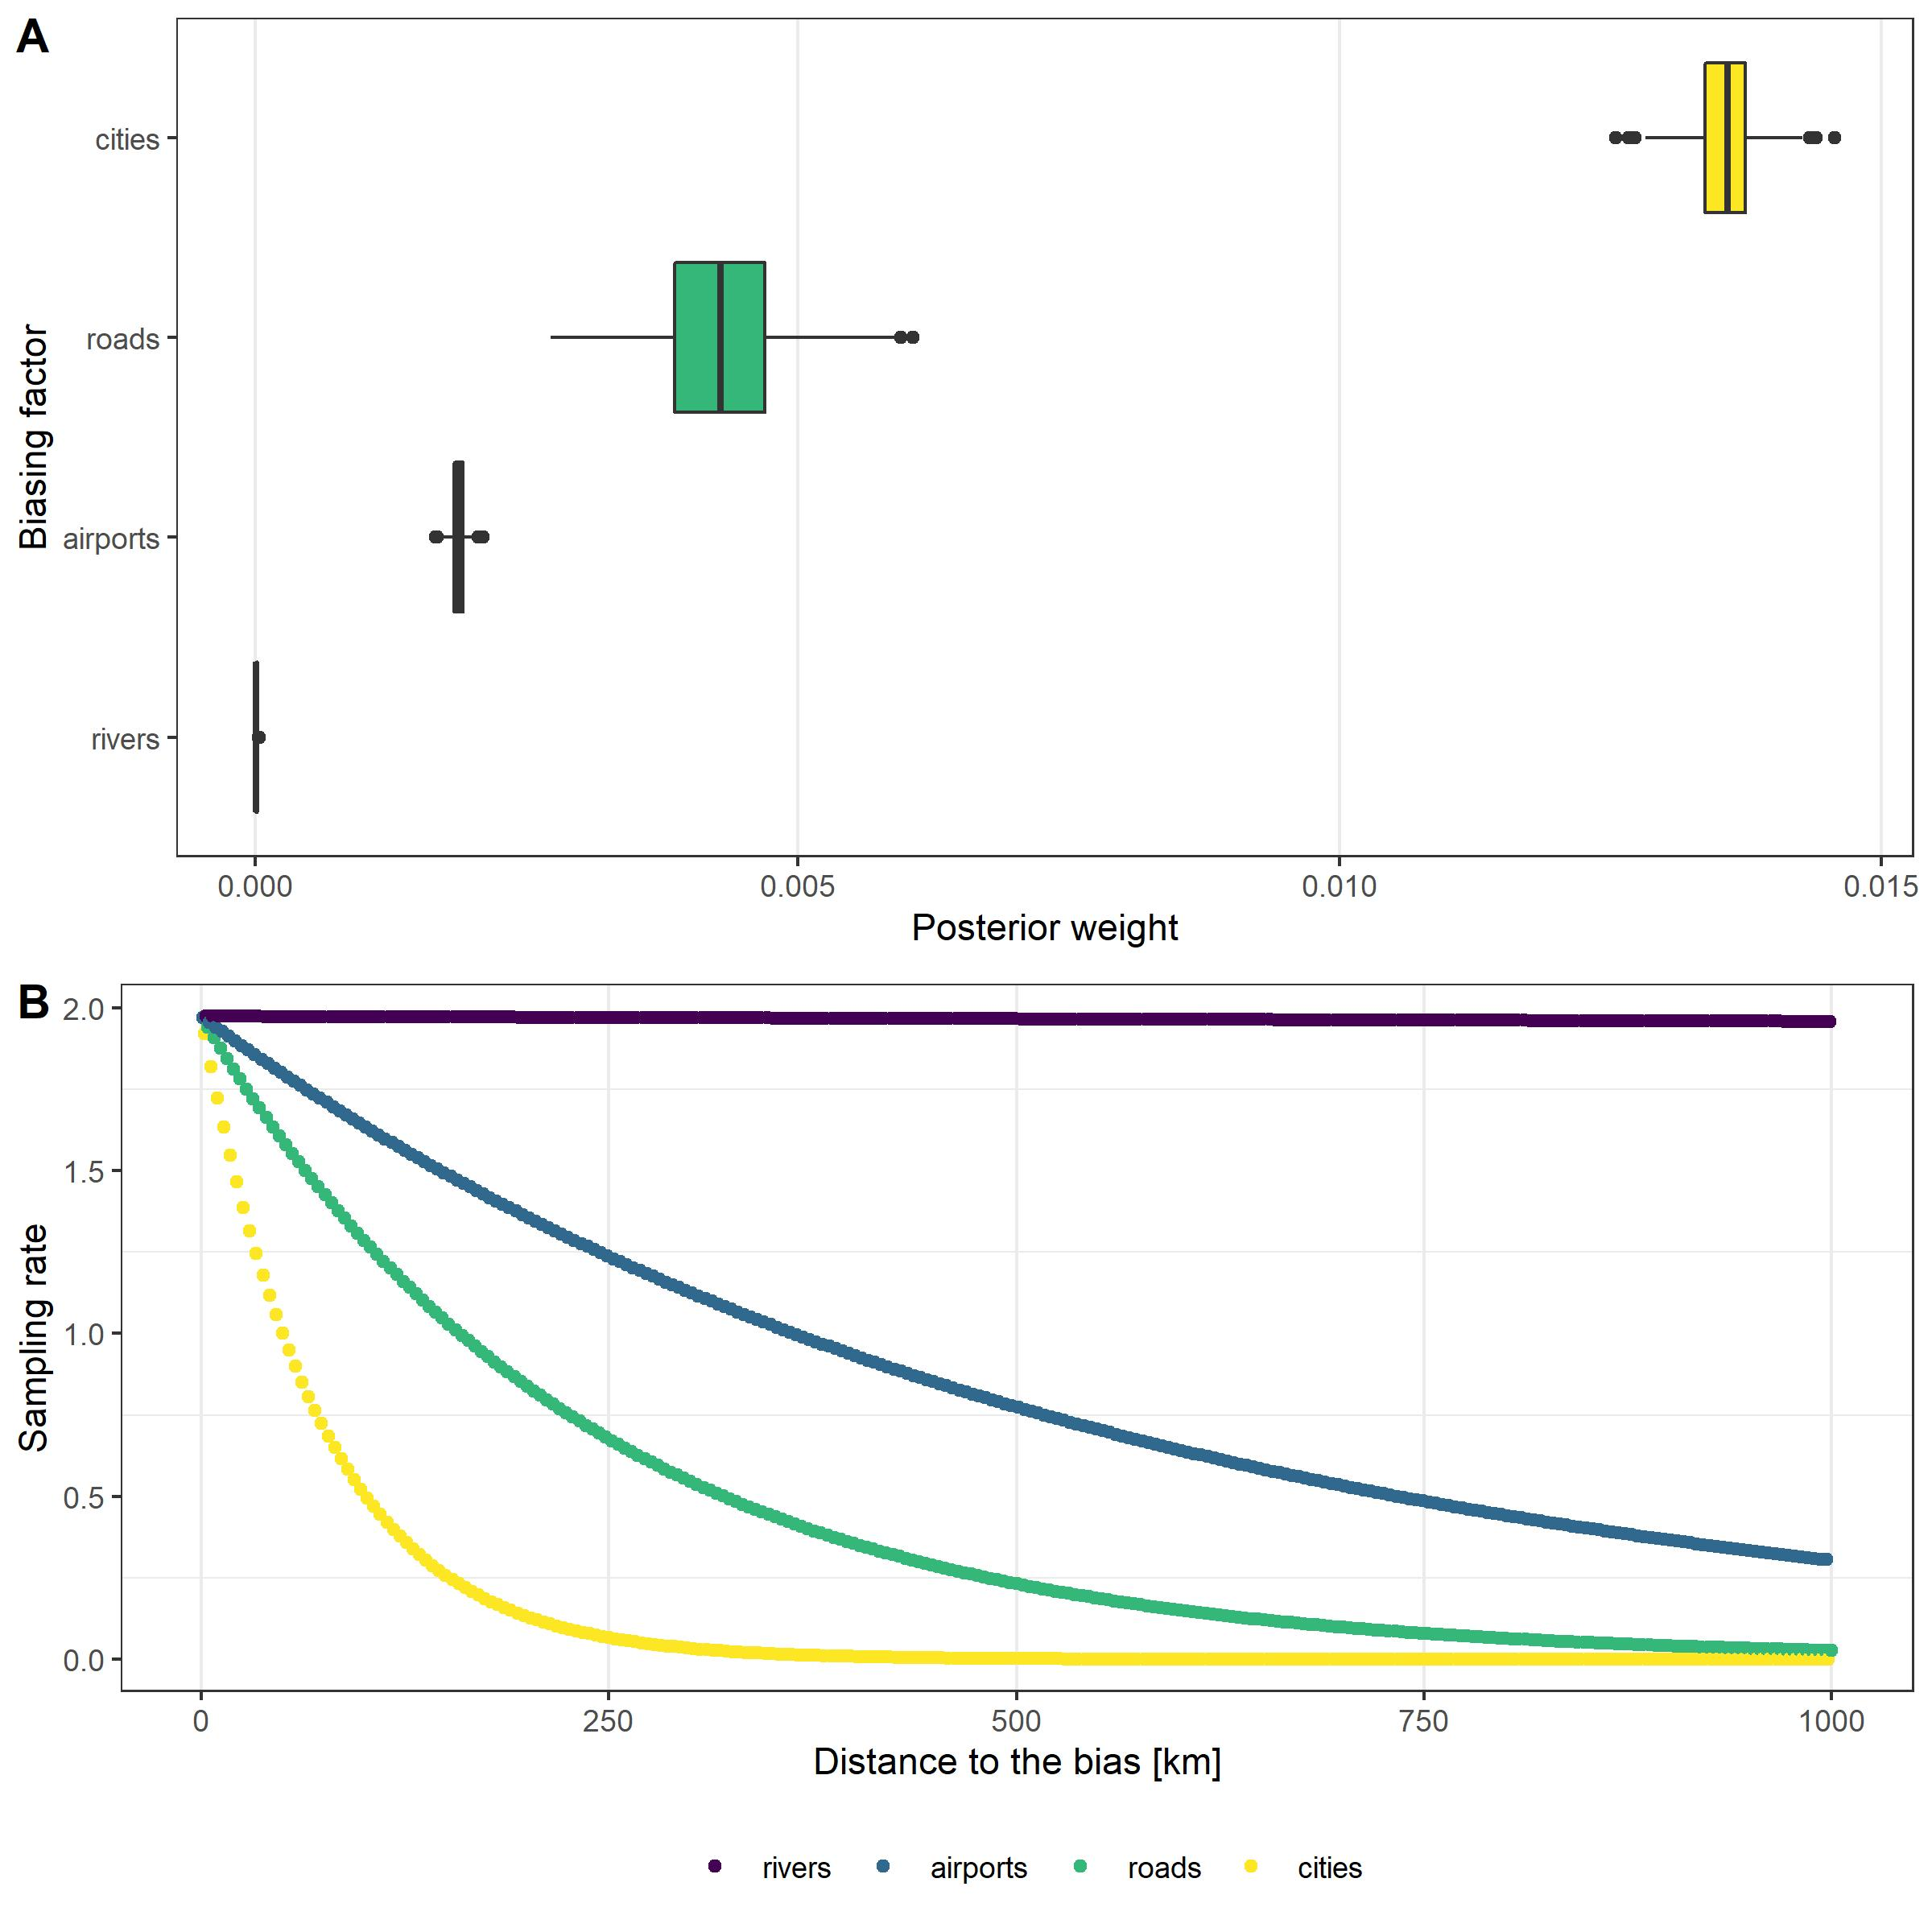
\includegraphics[width=6in]{ms_figures/figure_empirical_results} \caption{Results of the empirical validation analysis, estimating the accessibility bias in mammal occurrences from Borneo. A) bias weights ($w$) defining the effects of each bias factor, B) sampling rate as function of distance to the closest instance of each bias factor (the expected number of occurrences) given the inferred \textit{sampbias} model. At the study scale of 0.05 degrees (c. 5x5km) \textit{sampbias} finds the strongest biasing effect for the proximity of cities and roads.}\label{fig:empirical}
\end{figure}

\begin{figure}
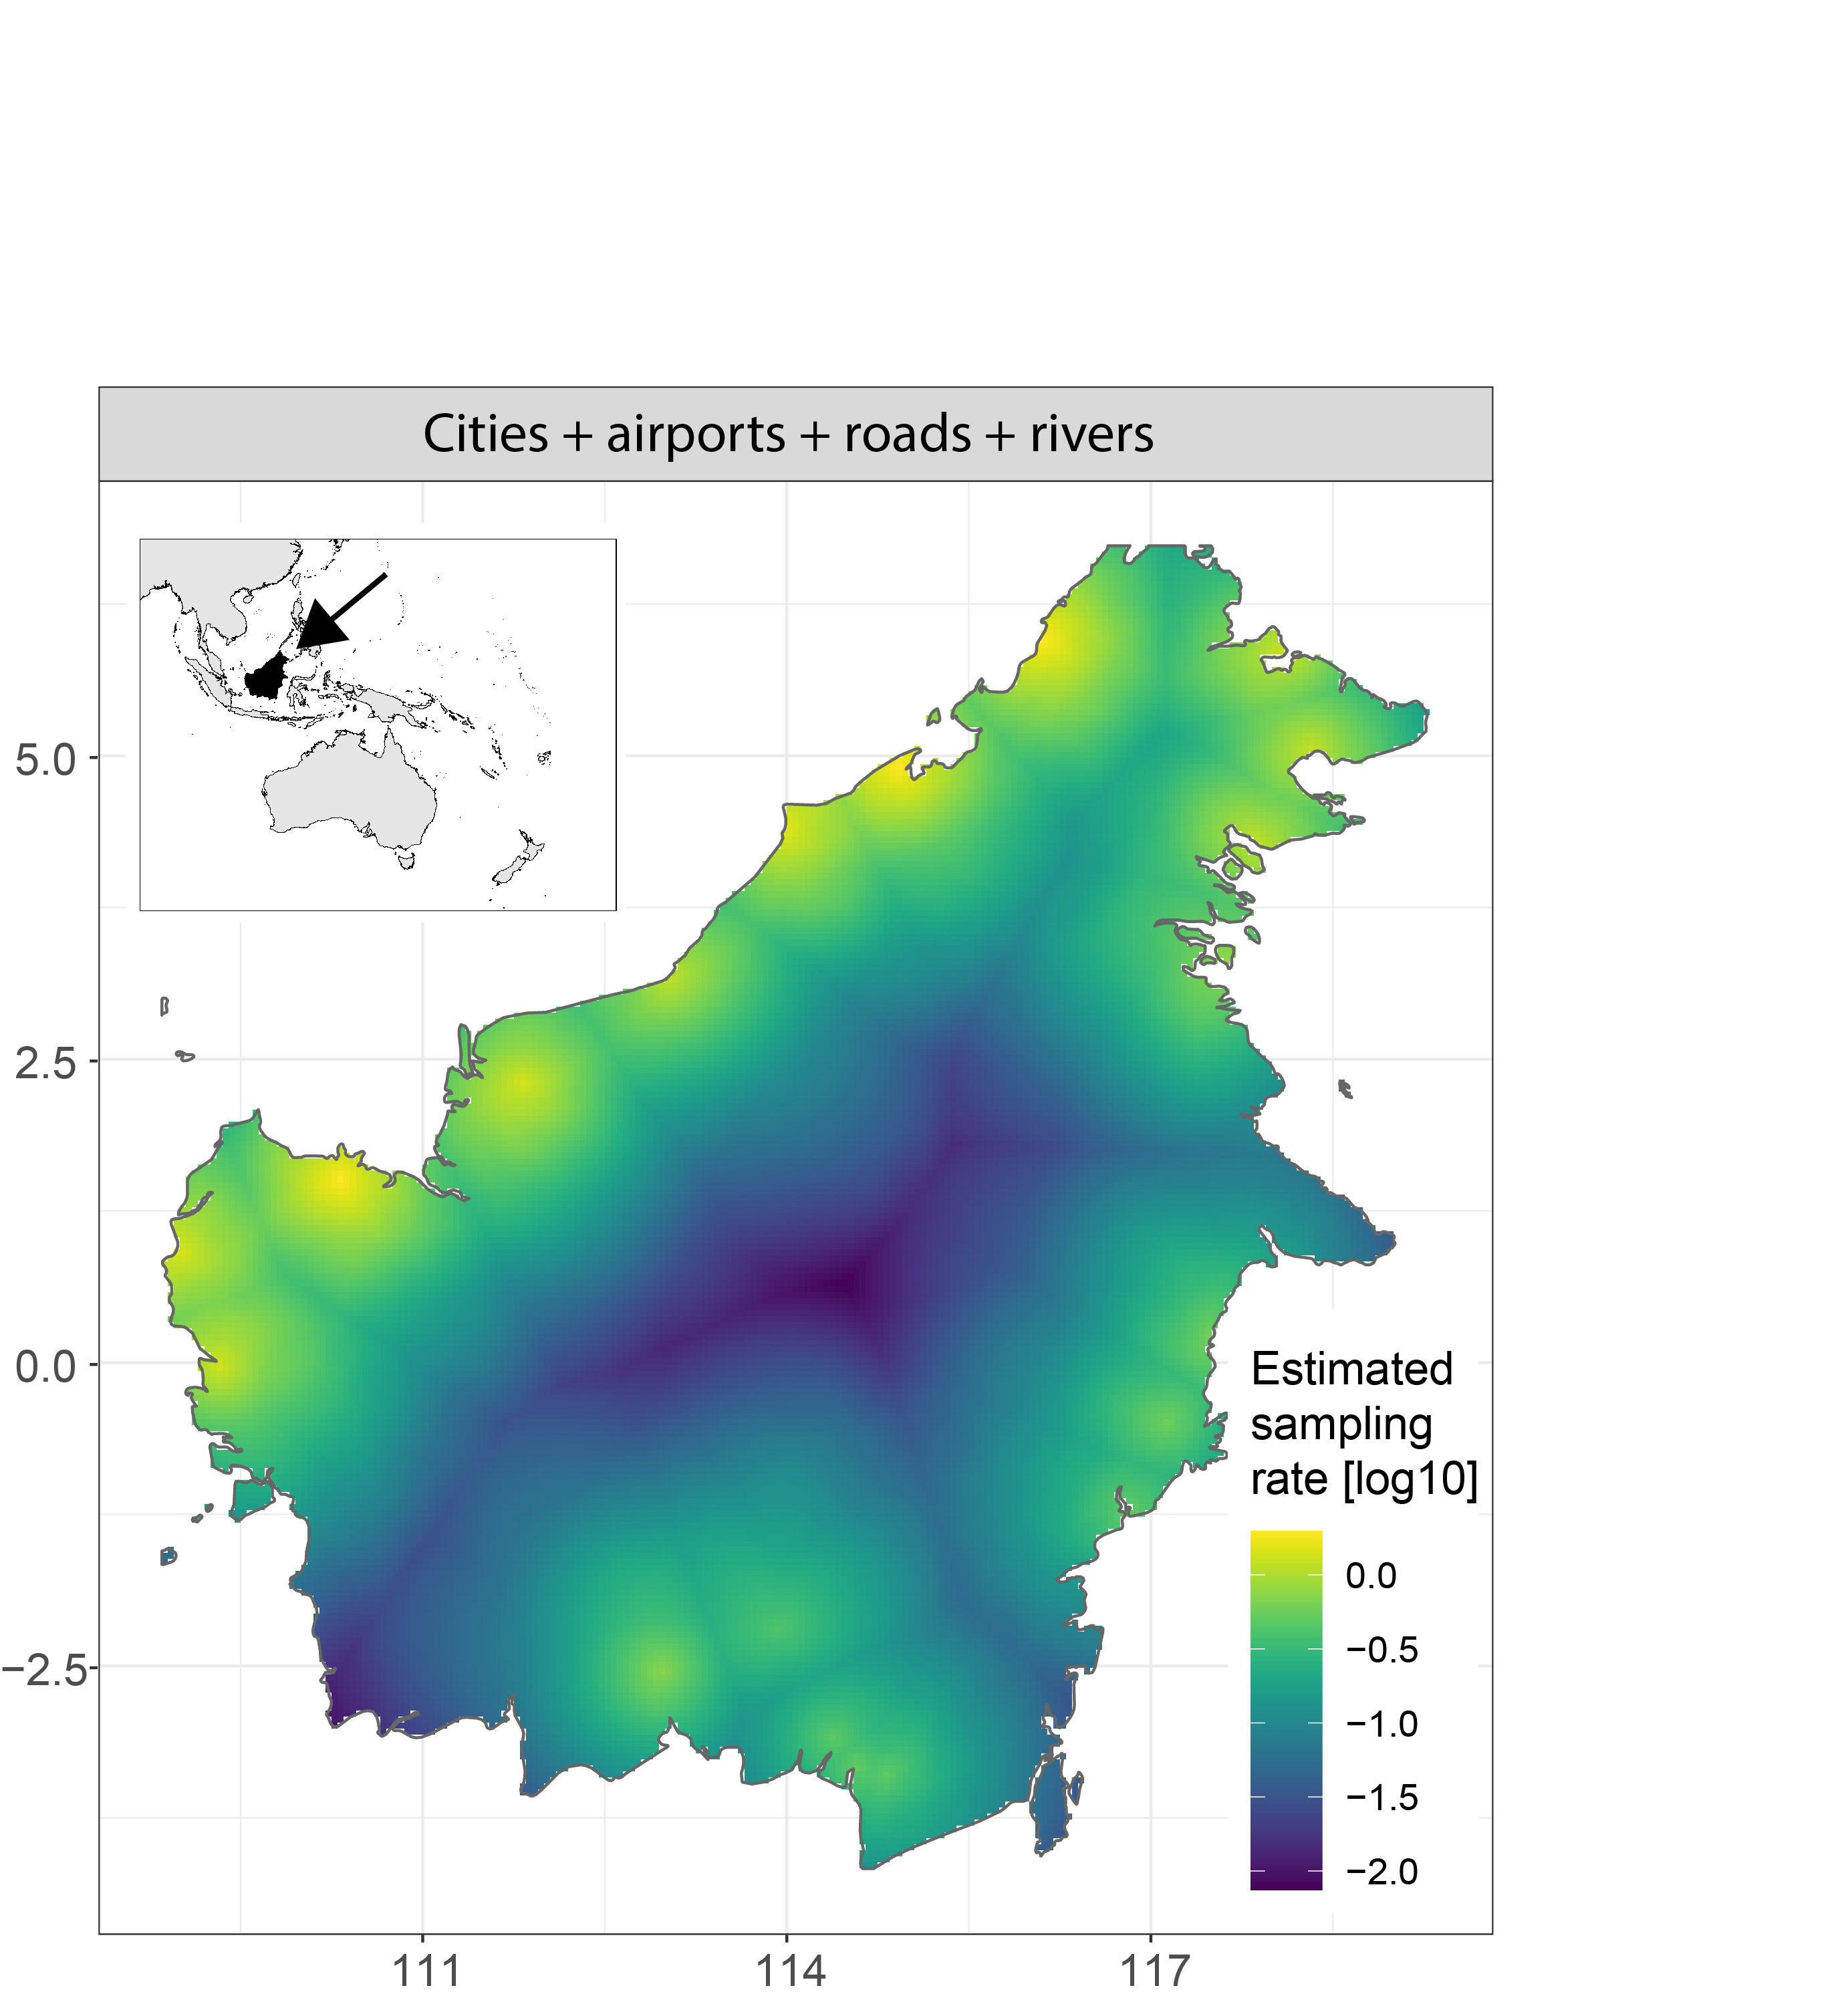
\includegraphics[width=6in]{ms_figures/figure_empirical_results_spatial_projection_adapted} \caption{Spatial projection of the sampling bias in an empirical example data set of mammal occurrences on the island of Borneo (downloaded from www.gbif.org. GBIF.org, 2016). The colours show the projection of the log10-transformed sampling rates (i.e. expected number of occurrences per cell) given the inferred \textit{sampbias} model. The highest undersampling is in the centre of the island. Different visualizations, including among others the untransformed sampling rate are also implemented in sampbias.}\label{fig:spatial}
\end{figure}

\newpage{}

\hypertarget{supplementary-material}{%
\section{Supplementary material}\label{supplementary-material}}

Appendix S1 - Tutorial running \emph{sampbias} in R

Appendix S2 - Supplementary Figures

Appendix S3 - Possible warnings and their solutions

\newpage{}

\hypertarget{references}{%
\section*{References}\label{references}}
\addcontentsline{toc}{section}{References}

\hypertarget{refs}{}
\leavevmode\hypertarget{ref-Aiello-Lammens2015}{}%
Aiello-Lammens, M. E. et al. 2015. spThin: An R package for spatial thinning of species occurrence records for use in ecological niche models. - Ecography 38: 541--545.

\leavevmode\hypertarget{ref-Bache2014}{}%
Bache, S. M. and Wickham, H. 2014. magrittr: A Forward-Pipe Operator for R.

\leavevmode\hypertarget{ref-Barbosa2013}{}%
Barbosa, A. M. et al. 2013. Species-people correlations and the need to account for survey effort in biodiversity analyses. - Diversity and Distributions 19: 1188--1197.

\leavevmode\hypertarget{ref-Beck2014}{}%
Beck, J. et al. 2014. Spatial bias in the GBIF database and its effect on modeling species' geographic distributions. - Ecological Informatics 19: 10--15.

\leavevmode\hypertarget{ref-Bivand2013}{}%
Bivand, R. S. et al. 2013. Applied spatial data analysis with R, Second edition. - Springer.

\leavevmode\hypertarget{ref-Boakes2010}{}%
Boakes, E. H. et al. 2010. Distorted views of biodiversity: Spatial and temporal bias in species occurrence data. - PLoS Biology 8: e1000385.

\leavevmode\hypertarget{ref-Boria2014}{}%
Boria, R. A. et al. 2014. Spatial filtering to reduce sampling bias can improve the performance of ecological niche models. - Ecological Modelling 275: 73--77.

\leavevmode\hypertarget{ref-Botts2011}{}%
Botts, E. A. et al. 2011. Geographic sampling bias in the South African Frog Atlas Project: Implications for conservation planning. - Biodiversity and Conservation 20: 119--139.

\leavevmode\hypertarget{ref-Bystriakova2012}{}%
Bystriakova, N. et al. 2012. Sampling bias in geographic and environmental space and its effect on the predictive power of species distribution models. - Systematics and Biodiversity 10: 305--315.

\leavevmode\hypertarget{ref-Daru2018}{}%
Daru, B. H. et al. 2018. Widespread sampling biases in herbaria revealed from large-scale digitization. - New Phytologist 217: 939--955.

\leavevmode\hypertarget{ref-Engemann2015}{}%
Engemann, K. et al. 2015. Limited sampling hampers ``big data'' estimation of species richness in a tropical biodiversity hotspot. - Ecology and Evolution 5: 807--820.

\leavevmode\hypertarget{ref-Fernandez2015}{}%
Fernández, D. and Nakamura, M. 2015. Estimation of spatial sampling effort based on presence-only data and accessibility. - Ecological Modelling 299: 147--155.

\leavevmode\hypertarget{ref-Fithian2014}{}%
Fithian, W. et al. 2015. Bias correction in species distribution models: pooling survey and collection data for multiple species. - Methods in Ecology and Evolution 6: 424--438.

\leavevmode\hypertarget{ref-Fourcade2014}{}%
Fourcade, Y. et al. 2014. Mapping species distributions with MAXENT using a geographically biased sample of presence data: A performance assessment of methods for correcting sampling bias. - PLoS ONE 9: e97122.

\leavevmode\hypertarget{ref-Garnier2018}{}%
Garnier, S. 2018. viridis: Default color maps from 'matplotlib'.

\leavevmode\hypertarget{ref-gbifdoi2016}{}%
GBIF.org 2016. (08 September 2016) GBIF occurrence download, doi.org/10.15468/dl.7fg4zx.

\leavevmode\hypertarget{ref-Hijmans2019}{}%
Hijmans, R. J. 2019. geosphere: Spherical Trigonometry.

\leavevmode\hypertarget{ref-Isaac2015}{}%
Isaac, N. J. B. and Pocock, M. J. O. 2015. Bias and information in biological records. - Biological Journal of the Linnean Society 115: 522--531.

\leavevmode\hypertarget{ref-Kadmon2004}{}%
Kadmon, R. et al. 2004. Effect of roadside bias on the accuracy of predictive maps produced by bioclimatic models. - Ecological Applications 14: 401--413.

\leavevmode\hypertarget{ref-Kery2016}{}%
Kery, M. and Royle, J. A. 2016. Applied hierarchical modeling in ecology - Analysis of distribution, abundance and species richness in R and BUGS: Volume 1: Prelude and Static Models. - Academic Press, Elsevier.

\leavevmode\hypertarget{ref-Komori2020}{}%
Komori, O. et al. 2020. Sampling bias correction in species distribution models by quasi-linear Poisson point process. - Ecological Informatics 55: 101015.

\leavevmode\hypertarget{ref-Kramer-Schadt2013}{}%
Kramer-Schadt, S. et al. 2013. The importance of correcting for sampling bias in MaxEnt species distribution models. - Diversity and Distributions 19: 1366--1379.

\leavevmode\hypertarget{ref-Lin2015}{}%
Lin, Y.-p. et al. 2015. Uncertainty analysis of crowd-sourced and professionally collected field data used in species distribution models of Taiwanese moths. - Biological Conservation 181: 102--110.

\leavevmode\hypertarget{ref-Lobo2011}{}%
Lobo, J. M. and Tognelli, M. F. 2011. Exploring the effects of quantity and location of pseudo-absences and sampling biases on the performance of distribution models with limited point occurrence data. - Journal for Nature Conservation 19: 1--7.

\leavevmode\hypertarget{ref-Meyer2015}{}%
Meyer, C. et al. 2015. Global priorities for an effective information basis of biodiversity distributions. - Nature Communications 6: 8221.

\leavevmode\hypertarget{ref-Meyer2016}{}%
Meyer, C. et al. 2016. Multidimensional biases, gaps and uncertainties in global plant occurrence information. - Ecology Letters 19: 992--1006.

\leavevmode\hypertarget{ref-Monsarrat2019}{}%
Monsarrat, S. et al. 2019. Accessibility maps as a tool to predict sampling bias in historical biodiversity occurrence records. - Ecography 42: 125--136.

\leavevmode\hypertarget{ref-Pebesma2005}{}%
Pebesma, E. J. and Bivand, R. S. 2005. Classes and methods for spatial Data: the sp Package. - R News 5: 21--41.

\leavevmode\hypertarget{ref-Phillips2009}{}%
Phillips, S. J. et al. 2009. Sample Selection Bias and Presence-Only Distribution Models : Implications for Background and Pseudo-Absence. - Ecological Applications 19: 181--197.

\leavevmode\hypertarget{ref-rcoreteam2019}{}%
R Core Team 2019. R: A language and environment for statistical computing.

\leavevmode\hypertarget{ref-Ruete2015}{}%
Ruete, A. 2015. Displaying bias in sampling effort of data accessed from biodiversity databases using ignorance maps. - Biodiversity Data Journal 3: e5361.

\leavevmode\hypertarget{ref-Ryden2019}{}%
Rydén, O. et al. 2020. Linking democracy and biodiversity conservation: Empirical evidence and research gaps. - Ambio 49: 419--433.

\leavevmode\hypertarget{ref-Shimadzu2015}{}%
Shimadzu, H. and Darnell, R. 2015. Attenuation of species abundance distributions by sampling. - Royal Society Open Science 2: 140219.

\leavevmode\hypertarget{ref-Stolar2015}{}%
Stolar, J. and Nielsen, S. E. 2015. Accounting for spatially biased sampling effort in presence-only species distribution modelling. - Diversity and Distributions 21: 595--608.

\leavevmode\hypertarget{ref-Vale2012}{}%
Vale, M. M. and Jenkins, C. N. 2012. Across-taxa incongruence in patterns of collecting bias. - Journal of Biogeography 39: 1744--1744.

\leavevmode\hypertarget{ref-Varela2014}{}%
Varela, S. et al. 2014. Environmental filters reduce the effects of sampling bias and improve predictions of ecological niche models. - Ecography 37: 1084--1091.

\leavevmode\hypertarget{ref-Wickham2009}{}%
Wickham, H. 2009. ggplot2 - Elegant graphics for data analysis. - Springer.

\leavevmode\hypertarget{ref-Wickham2019b}{}%
Wickham, H. 2019. forcats: Tools for working with categorical variables (Factors).

\leavevmode\hypertarget{ref-Wickham2019a}{}%
Wickham, H. and Henry, L. 2019. tidyr: Tidy messy data.

\leavevmode\hypertarget{ref-Wickham2019}{}%
Wickham, H. et al. 2019. dplyr: A grammar of data manipulation.

\leavevmode\hypertarget{ref-Yang2013}{}%
Yang, W. et al. 2013. Geographical sampling bias in a large distributional database and its effects on species richness-environment models. - Journal of Biogeography 40: 1415--1426.

\leavevmode\hypertarget{ref-Yang2014}{}%
Yang, W. et al. 2014. Environmental and socio-economic factors shaping the geography of floristic collections in China. - Global Ecology and Biogeography 23: 1284--1292.

\leavevmode\hypertarget{ref-Zizka2020c}{}%
Zizka, A. et al. 2020. Exploring the Impact of Political Regimes on Biodiversity. - VDem working papers 98: 1--13.

\end{document}
